\documentclass[12pt]{article}
\usepackage[utf8]{inputenc}
\usepackage{xcolor}
\usepackage[margin=1in]{geometry}
% \usepackage{graphicx}
\usepackage{float}
% \usepackage{textcomp}
% \usepackage{siunitx}
\usepackage{fancyhdr}
% \usepackage{amsmath, amssymb, amsthm}
\usepackage{tikz}
\usepackage{tikzpagenodes}
% \usepackage{eso-pic}
% \usepackage{enumerate}
\usepackage[colorlinks]{hyperref}
\hypersetup{
    colorlinks = true,
    linkcolor = blue,
    pdftitle={Graph Theory and Algorithms}
}
% \usepackage{lipsum}
% \usepackage{etoolbox}
\usepackage{bookmark}

% \makeatletter

% \renewcommand\float@endH{\@endfloatbox\vskip\intextsep
%   \if@flstyle\setbox\@currbox\float@makebox\columnwidth\fi
%   \box\@currbox\vskip\intextsep\relax\@doendpe}

% \patchcmd{\f@nch@head}{\rlap}{\color{white}\rlap}{}{}
% \patchcmd{\headrule}{\hrule}{\color{white}\hrule}{}{}
% \patchcmd{\f@nch@foot}{\rlap}{\color{white}\rlap}{}{}
% \patchcmd{\footrule}{\hrule}{\color{white}\hrule}{}{}

% \makeatother

%%% Header and footer
%%% ------------------------------------------
\pagestyle{fancy}
\fancyhf{}
\rhead{Summer of Science: Graph Theory}
% \fancyhead[L]{\nouppercase{\leftmark}}
\cfoot{\thepage}

%%% Macros
%%% ------------------------------------------
% \newcommand{\desctotoc}[4]{%
%   \addtocontents{toc}{\medskip\noindent\detokenize{#1}\leavevmode\par\medskip}
% }


\begin{document}


%%% Titlepage
%%% ------------------------------------------
\tikz[overlay] \node[opacity=1,inner sep=0pt] at (7.65,-12.5) {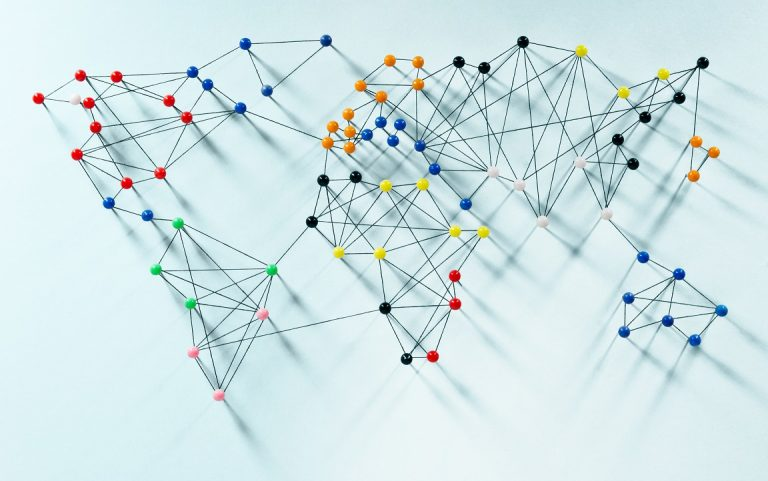
\includegraphics[width=\paperwidth]{./Graph-Theory-768x481.jpg}};
\vspace*{3cm}
\thispagestyle{empty}
	\begin{center}
	\textbf{\Huge{Graph Theory and Algorithms}}\\
	\textbf{\large{\\ An Introduction to the world of Graphs }}
	\end{center}
\vfill
	\begin{center}
	\large{\textbf{Devansh Jain,}\\
    Indian Institute of Technology, Bombay\\
    \vspace{0.5cm}
    (Mentor: Tathagat Verma)\\}
	\end{center}

\newpage

%%% Table of Contents
%%% ------------------------------------------
\pagenumbering{roman}
\begin{center}
\hspace{0pt}
    \tableofcontents
    \vfill
\hspace{0pt}
\end{center}

\newpage

\section*{Preface}
\addcontentsline{toc}{section}{Preface}
Preface
\subsubsection*{About the project}
adedsd
\subsubsection*{About the report}
sdsd
\subsubsection*{References and Acknowledgement}
sdfsd


\newpage
\pagenumbering{Roman}
\setcounter{page}{1}
{\color{black} \section*{MIT 6.042J}}
\addcontentsline{toc}{section}{MIT 6.042J}
About it
\newpage
\pagenumbering{arabic}
\setcounter{page}{23}
\newpage
\begin{figure}[H]
    \centering
    \includegraphics[scale=0.25]{"./MIT 6.042J/MIT_6042J_023"}
\end{figure}
\newpage
\begin{figure}[H]
    \centering
    \includegraphics[scale=0.25]{"./MIT 6.042J/MIT_6042J_024"}
\end{figure}
\newpage
\begin{figure}[H]
    \centering
    \includegraphics[scale=0.25]{"./MIT 6.042J/MIT_6042J_025"}
\end{figure}
\newpage
\begin{figure}[H]
    \centering
    \includegraphics[scale=0.25]{"./MIT 6.042J/MIT_6042J_026"}
\end{figure}
\newpage
\begin{figure}[H]
    \centering
    \includegraphics[scale=0.25]{"./MIT 6.042J/MIT_6042J_027"}
\end{figure}
\newpage
\begin{figure}[H]
    \centering
    \includegraphics[scale=0.25]{"./MIT 6.042J/MIT_6042J_028"}
\end{figure}
\newpage
\begin{figure}[H]
    \centering
    \includegraphics[scale=0.25]{"./MIT 6.042J/MIT_6042J_029"}
\end{figure}
\newpage
\begin{figure}[H]
    \centering
    \includegraphics[scale=0.25]{"./MIT 6.042J/MIT_6042J_030"}
\end{figure}
\newpage
\begin{figure}[H]
    \centering
    \includegraphics[scale=0.25]{"./MIT 6.042J/MIT_6042J_031"}
\end{figure}
\newpage
\begin{figure}[H]
    \centering
    \includegraphics[scale=0.25]{"./MIT 6.042J/MIT_6042J_032"}
\end{figure}
\newpage
\begin{figure}[H]
    \centering
    \includegraphics[scale=0.25]{"./MIT 6.042J/MIT_6042J_033"}
\end{figure}
\newpage
\begin{figure}[H]
    \centering
    \includegraphics[scale=0.25]{"./MIT 6.042J/MIT_6042J_034"}
\end{figure}
\newpage
\begin{figure}[H]
    \centering
    \includegraphics[scale=0.25]{"./MIT 6.042J/MIT_6042J_035"}
\end{figure}
\newpage
\begin{figure}[H]
    \centering
    \includegraphics[scale=0.25]{"./MIT 6.042J/MIT_6042J_036"}
\end{figure}
\newpage
\begin{figure}[H]
    \centering
    \includegraphics[scale=0.25]{"./MIT 6.042J/MIT_6042J_037"}
\end{figure}
\newpage
\begin{figure}[H]
    \centering
    \includegraphics[scale=0.25]{"./MIT 6.042J/MIT_6042J_038"}
\end{figure}
\newpage
\begin{figure}[H]
    \centering
    \includegraphics[scale=0.25]{"./MIT 6.042J/MIT_6042J_039"}
\end{figure}
\newpage
\begin{figure}[H]
    \centering
    \includegraphics[scale=0.25]{"./MIT 6.042J/MIT_6042J_040"}
\end{figure}
\newpage
\begin{figure}[H]
    \centering
    \includegraphics[scale=0.25]{"./MIT 6.042J/MIT_6042J_041"}
\end{figure}
\newpage
\begin{figure}[H]
    \centering
    \includegraphics[scale=0.25]{"./MIT 6.042J/MIT_6042J_042"}
\end{figure}
\newpage
\begin{figure}[H]
    \centering
    \includegraphics[scale=0.25]{"./MIT 6.042J/MIT_6042J_043"}
\end{figure}
\newpage
\begin{figure}[H]
    \centering
    \includegraphics[scale=0.25]{"./MIT 6.042J/MIT_6042J_044"}
\end{figure}
\newpage
\begin{figure}[H]
    \centering
    \includegraphics[scale=0.25]{"./MIT 6.042J/MIT_6042J_045"}
\end{figure}
\newpage
\begin{figure}[H]
    \centering
    \includegraphics[scale=0.25]{"./MIT 6.042J/MIT_6042J_046"}
\end{figure}
\newpage
\begin{figure}[H]
    \centering
    \includegraphics[scale=0.25]{"./MIT 6.042J/MIT_6042J_047"}
\end{figure}
\newpage
\begin{figure}[H]
    \centering
    \includegraphics[scale=0.25]{"./MIT 6.042J/MIT_6042J_048"}
\end{figure}
\newpage
\begin{figure}[H]
    \centering
    \includegraphics[scale=0.25]{"./MIT 6.042J/MIT_6042J_049"}
\end{figure}
\newpage
\begin{figure}[H]
    \centering
    \includegraphics[scale=0.25]{"./MIT 6.042J/MIT_6042J_050"}
\end{figure}
\newpage
\begin{figure}[H]
    \centering
    \includegraphics[scale=0.25]{"./MIT 6.042J/MIT_6042J_051"}
\end{figure}
\newpage
\begin{figure}[H]
    \centering
    \includegraphics[scale=0.25]{"./MIT 6.042J/MIT_6042J_052"}
\end{figure}
\newpage
\begin{figure}[H]
    \centering
    \includegraphics[scale=0.25]{"./MIT 6.042J/MIT_6042J_053"}
\end{figure}
\newpage
\begin{figure}[H]
    \centering
    \includegraphics[scale=0.25]{"./MIT 6.042J/MIT_6042J_054"}
\end{figure}
\newpage
\begin{figure}[H]
    \centering
    \includegraphics[scale=0.25]{"./MIT 6.042J/MIT_6042J_055"}
\end{figure}
\newpage
\begin{figure}[H]
    \centering
    \includegraphics[scale=0.25]{"./MIT 6.042J/MIT_6042J_056"}
\end{figure}
\newpage
\begin{figure}[H]
    \centering
    \includegraphics[scale=0.25]{"./MIT 6.042J/MIT_6042J_057"}
\end{figure}
\newpage
\begin{figure}[H]
    \centering
    \includegraphics[scale=0.25]{"./MIT 6.042J/MIT_6042J_058"}
\end{figure}
\newpage
\begin{figure}[H]
    \centering
    \includegraphics[scale=0.25]{"./MIT 6.042J/MIT_6042J_059"}
\end{figure}
\newpage
\begin{figure}[H]
    \centering
    \includegraphics[scale=0.25]{"./MIT 6.042J/MIT_6042J_060"}
\end{figure}
\newpage
\begin{figure}[H]
    \centering
    \includegraphics[scale=0.25]{"./MIT 6.042J/MIT_6042J_061"}
\end{figure}
\newpage
\begin{figure}[H]
    \centering
    \includegraphics[scale=0.25]{"./MIT 6.042J/MIT_6042J_062"}
\end{figure}
\newpage
\begin{figure}[H]
    \centering
    \includegraphics[scale=0.25]{"./MIT 6.042J/MIT_6042J_063"}
\end{figure}
\newpage
\begin{figure}[H]
    \centering
    \includegraphics[scale=0.25]{"./MIT 6.042J/MIT_6042J_064"}
\end{figure}
\newpage
\begin{figure}[H]
    \centering
    \includegraphics[scale=0.25]{"./MIT 6.042J/MIT_6042J_065"}
\end{figure}
\newpage
\begin{figure}[H]
    \centering
    \includegraphics[scale=0.25]{"./MIT 6.042J/MIT_6042J_066"}
\end{figure}
\newpage
\begin{figure}[H]
    \centering
    \includegraphics[scale=0.25]{"./MIT 6.042J/MIT_6042J_067"}
\end{figure}
\newpage
\begin{figure}[H]
    \centering
    \includegraphics[scale=0.25]{"./MIT 6.042J/MIT_6042J_068"}
\end{figure}
\newpage
\begin{figure}[H]
    \centering
    \includegraphics[scale=0.25]{"./MIT 6.042J/MIT_6042J_069"}
\end{figure}
\newpage
\begin{figure}[H]
    \centering
    \includegraphics[scale=0.25]{"./MIT 6.042J/MIT_6042J_070"}
\end{figure}
\newpage
\begin{figure}[H]
    \centering
    \includegraphics[scale=0.25]{"./MIT 6.042J/MIT_6042J_071"}
\end{figure}
\newpage
\begin{figure}[H]
    \centering
    \includegraphics[scale=0.25]{"./MIT 6.042J/MIT_6042J_072"}
\end{figure}
\newpage
\begin{figure}[H]
    \centering
    \includegraphics[scale=0.25]{"./MIT 6.042J/MIT_6042J_073"}
\end{figure}
\newpage
\begin{figure}[H]
    \centering
    \includegraphics[scale=0.25]{"./MIT 6.042J/MIT_6042J_074"}
\end{figure}
\newpage
\begin{figure}[H]
    \centering
    \includegraphics[scale=0.25]{"./MIT 6.042J/MIT_6042J_075"}
\end{figure}
\newpage
\begin{figure}[H]
    \centering
    \includegraphics[scale=0.25]{"./MIT 6.042J/MIT_6042J_076"}
\end{figure}
\newpage
\begin{figure}[H]
    \centering
    \includegraphics[scale=0.25]{"./MIT 6.042J/MIT_6042J_077"}
\end{figure}

% {\color{black} \subsubsection*{Lecture 6: Intro to Graphs}}
% \addcontentsline{toc}{subsection}{Lecture 6: Intro to Graphs}
% \begin{figure}[H]
%     \centering
%     \includegraphics[width=16cm, height=20cm]{"./MIT-6.042J/MIT-6042J-023"}
% \end{figure}
% \newpage
% {\color{black} \subsubsection*{Lecture 6: Intro to Graphs}}
% % \addcontentsline{toc}{subsection}{Lecture 6: Intro to Graphs}
% \begin{figure}[H]
%     \centering
%     \includegraphics[width=16cm, height=21cm]{"./MIT-6.042J/MIT-6042J-024"}
% \end{figure}
% \newpage
% {\color{black} \subsubsection*{Lecture 6: Intro to Graphs}}
% % \addcontentsline{toc}{subsection}{Lecture 6: Intro to Graphs}
% \begin{figure}[H]
%     \centering
%     \includegraphics[width=16cm, height=21cm]{"./MIT-6.042J/MIT-6042J-025"}
% \end{figure}

\newpage

\section{MIT 6.006}
\newpage
\begin{figure}[H]
    \centering
    \includegraphics[scale=0.25]{"./MIT-6.006/MIT-6006-095"}
\end{figure}
\newpage
\begin{figure}[H]
    \centering
    \includegraphics[scale=0.25]{"./MIT-6.006/MIT-6006-096"}
\end{figure}
\newpage
\begin{figure}[H]
    \centering
    \includegraphics[scale=0.25]{"./MIT-6.006/MIT-6006-097"}
\end{figure}
\newpage
\begin{figure}[H]
    \centering
    \includegraphics[scale=0.25]{"./MIT-6.006/MIT-6006-098"}
\end{figure}
\newpage
\begin{figure}[H]
    \centering
    \includegraphics[scale=0.25]{"./MIT-6.006/MIT-6006-099"}
\end{figure}
\newpage
\begin{figure}[H]
    \centering
    \includegraphics[scale=0.25]{"./MIT-6.006/MIT-6006-100"}
\end{figure}
\newpage
\begin{figure}[H]
    \centering
    \includegraphics[scale=0.25]{"./MIT-6.006/MIT-6006-101"}
\end{figure}
\newpage
\begin{figure}[H]
    \centering
    \includegraphics[scale=0.25]{"./MIT-6.006/MIT-6006-102"}
\end{figure}
\newpage
\begin{figure}[H]
    \centering
    \includegraphics[scale=0.25]{"./MIT-6.006/MIT-6006-103"}
\end{figure}
\newpage
\begin{figure}[H]
    \centering
    \includegraphics[scale=0.25]{"./MIT-6.006/MIT-6006-104"}
\end{figure}
\newpage
\begin{figure}[H]
    \centering
    \includegraphics[scale=0.25]{"./MIT-6.006/MIT-6006-105"}
\end{figure}
\newpage
\begin{figure}[H]
    \centering
    \includegraphics[scale=0.25]{"./MIT-6.006/MIT-6006-106"}
\end{figure}
\newpage
\begin{figure}[H]
    \centering
    \includegraphics[scale=0.25]{"./MIT-6.006/MIT-6006-107"}
\end{figure}
\newpage
\begin{figure}[H]
    \centering
    \includegraphics[scale=0.25]{"./MIT-6.006/MIT-6006-108"}
\end{figure}
\newpage
\begin{figure}[H]
    \centering
    \includegraphics[scale=0.25]{"./MIT-6.006/MIT-6006-109"}
\end{figure}
\newpage
\begin{figure}[H]
    \centering
    \includegraphics[scale=0.25]{"./MIT-6.006/MIT-6006-110"}
\end{figure}
\newpage
\begin{figure}[H]
    \centering
    \includegraphics[scale=0.25]{"./MIT-6.006/MIT-6006-111"}
\end{figure}
\newpage
\begin{figure}[H]
    \centering
    \includegraphics[scale=0.25]{"./MIT-6.006/MIT-6006-112"}
\end{figure}
\newpage
\begin{figure}[H]
    \centering
    \includegraphics[scale=0.25]{"./MIT-6.006/MIT-6006-113"}
\end{figure}
\newpage
\begin{figure}[H]
    \centering
    \includegraphics[scale=0.25]{"./MIT-6.006/MIT-6006-114"}
\end{figure}
\newpage
\begin{figure}[H]
    \centering
    \includegraphics[scale=0.25]{"./MIT-6.006/MIT-6006-115"}
\end{figure}
\newpage
\begin{figure}[H]
    \centering
    \includegraphics[scale=0.25]{"./MIT-6.006/MIT-6006-116"}
\end{figure}
\newpage
\begin{figure}[H]
    \centering
    \includegraphics[scale=0.25]{"./MIT-6.006/MIT-6006-117"}
\end{figure}
\newpage
\begin{figure}[H]
    \centering
    \includegraphics[scale=0.25]{"./MIT-6.006/MIT-6006-118"}
\end{figure}
\newpage
\begin{figure}[H]
    \centering
    \includegraphics[scale=0.25]{"./MIT-6.006/MIT-6006-119"}
\end{figure}
\newpage
\begin{figure}[H]
    \centering
    \includegraphics[scale=0.25]{"./MIT-6.006/MIT-6006-120"}
\end{figure}
\newpage
\begin{figure}[H]
    \centering
    \includegraphics[scale=0.25]{"./MIT-6.006/MIT-6006-121"}
\end{figure}
\newpage
\begin{figure}[H]
    \centering
    \includegraphics[scale=0.25]{"./MIT-6.006/MIT-6006-122"}
\end{figure}
\newpage
\begin{figure}[H]
    \centering
    \includegraphics[scale=0.25]{"./MIT-6.006/MIT-6006-123"}
\end{figure}
\newpage
\begin{figure}[H]
    \centering
    \includegraphics[scale=0.25]{"./MIT-6.006/MIT-6006-124"}
\end{figure}
\newpage
\begin{figure}[H]
    \centering
    \includegraphics[scale=0.25]{"./MIT-6.006/MIT-6006-125"}
\end{figure}
\newpage
\begin{figure}[H]
    \centering
    \includegraphics[scale=0.25]{"./MIT-6.006/MIT-6006-126"}
\end{figure}
\newpage
\begin{figure}[H]
    \centering
    \includegraphics[scale=0.25]{"./MIT-6.006/MIT-6006-127"}
\end{figure}
\newpage
\begin{figure}[H]
    \centering
    \includegraphics[scale=0.25]{"./MIT-6.006/MIT-6006-128"}
\end{figure}
\newpage
\begin{figure}[H]
    \centering
    \includegraphics[scale=0.25]{"./MIT-6.006/MIT-6006-129"}
\end{figure}
\newpage
\begin{figure}[H]
    \centering
    \includegraphics[scale=0.25]{"./MIT-6.006/MIT-6006-130"}
\end{figure}
\newpage
\begin{figure}[H]
    \centering
    \includegraphics[scale=0.25]{"./MIT-6.006/MIT-6006-131"}
\end{figure}
\newpage
\begin{figure}[H]
    \centering
    \includegraphics[scale=0.25]{"./MIT-6.006/MIT-6006-132"}
\end{figure}
\newpage
\begin{figure}[H]
    \centering
    \includegraphics[scale=0.25]{"./MIT-6.006/MIT-6006-133"}
\end{figure}


% \section{Variable Stars and their Types}
% Let us take a break from some intensive mathematics and look at a special category of stars. This sections is purely descriptive, and we shall deal with the state dynamics of these stars later in the article.
\subsection{Causes of Variation}
The light output of virtually every star, including our Sun, varies over time, form a period of minutes to several billion years. Both causes and manifestations are many and varied; a recent count identified more than 70 classes of variable stars, most of the names after the first star (called prototype) in which it was first observed. Let us take a look at some of these types and their probable causes.
\subsubsection{Pulsational Variables}
These are the most useful variable stars because the length of time in which they brighten and fade again, i.e. their periods, are frequently correlated with their absolute brightness, so that they can be used to measure distances to star clusters anywhere in the Milky Way and to nearby galaxies.
\begin{figure}[H]
    \centering
    \color{white}
    \includegraphics[scale=1]{RRL.jpg}
    \caption{The galactic centre view showing multiple RR Lyrae variables, that help us determine the distance to it}
    \label{fig:my_label}
\end{figure}
\noindent
Their pulsation might be driven by some instability, and the restoring force that brings the gas back where it started from can be gravity or pressure or magnetic fields. In this sense, the instability is intrinsic to the star and not due to external influences; hence, such stars are often referred to as intrinsic variables. The type of instability and the restoring force employed by the star can be used to differentiate between different types of variables, some of the more common ones being:
\begin{itemize}
    \item \textit{Classical Cepheids}, usually just called Cepheids are young, metal rich stars with periods of days to months. They appear to be purely radial pulsators.
    \item \textit{RR Lyrae} variables were formerly known as cluster type variables or cluster Cepheids because they are common in globular clusters. They have periods of a day down to a couple of hours and are useful in determine distances to globular clusters in out galaxy in nearby galaxies.
    \item $\delta$ \textit{Scruti} variables have periods ranging from about 30 minutes to 8 hours and pulsate in radial and non-radial pressure nodes although gravity may be present. Amplitudes tend to be low.
    \item \textit{Mira} variables, are luminours red supergiants belonging in the class of \textit{Long Period Variables} with periods ranging from roughly 100 to 700 days. Radial nodes seem to be the norm.  \textit{RV Tauri} stars are an extreme version with low mass and large luminosity, so that a second pulse starts before the atmosphere has had time to fall down from the previous one.
    \item \textit{The Rapidly Oscillating Ap} stars are characterized by low amplitude, short period photometric variations, typically 10 minutes, strong magnetic fields, and enhanced surface abundances of exotic elements such as strontium and europium. The observed light variations are modulated in amplitude by the rotation of the star and it is thought that the pulsations are carried around by an off-axis magnetic field as the star rotates.
\end{itemize}
\begin{figure}[H]
    \centering
    \color{white}
    \includegraphics[scale=0.5]{cepheid.png}
    \caption{Light curves of four different cepheids showing how the light output varies with time}
    \label{fig:my_label}
\end{figure}
\noindent
\subsubsection{Explosive variables}
These are the stars that release a great deal of nuclear or gravitational energy in a hurry. The cataclysmic variables are close star pairs with a white dwarf in orbit with a main sequence or red giant companion. The white dwarf accepts material from its companion, One sort of variability arises when the rate of acceptance or accretion and therefore the rate of release of gravitational potential energy changes. When enough hydrogen-rich material has accumulated on the surface of the white dwarf it fuses explosively.\\\\
\textbf{Novae}\\\\
Nova is the name given to these outbursts fueled by degenerate hydrogen ignition.
\begin{figure}[H]
    \centering
    \color{white}
    \includegraphics[scale=0.5]{nova.png}
    \caption{Light output curve for a typical nova as is explained below}
    \label{fig:my_label}
\end{figure}
\noindent
As seen above, there is a fast rise lasting perhaps a day, followed by a decline in brightness that may be quite variable from nova to nova. In the ``fast" novae the decline may take a couple of weeks to reduce the visual brightness by two magnitudes. ``Slow" novae may take a few months to accomplish the same thing. Between the initial rise and eventual decline, there may be a plateau near the peak lasting an hour or so in fast novae but extending over days in slow ones. As indicated in the figure, the decline phase may be interrupted by oscillations or a pronounced trough. \\\\
\textbf{Supernovae}\\\\
Supernovae are the most spectacular variables of all. At maximum light, they are as bright as a whole, smallish galaxy, and recognizing them for what they are was part of the total process between 1900-1925 CE that sorted out the approximate size of the Milky Way and demonstrated the existence of other galaxies. There is a sort of family resemblance among all supernovae - they get really bright in a matter of days and fade in months to years. Their spectra display very broad features, indicating velocities of thousands of km s$^{-1}$. And they blow out a solar mass or more of material at these large velocities that can then be seen as supernova remnant for thousands of years thereafter. We shall not get into much more detail because the dynamics of supernovae is beyond the scope of this article.
\begin{figure}[H]
    \centering
    \color{white}
    \includegraphics[scale=0.5]{supernova.jpg}
    \caption{Crab nebula: a supernova remnant in Taurus}
    \label{fig:my_label}
\end{figure}
\noindent
\subsection{Other Broad Categories of Variables}
As mentioned in the beginning of this section, every star shows some kind of variability upon observation, which may be intrinsic or may be due to purely observational factors. These may not be as ``interesting" as pulsational or explosive variables, but they are significant and worth mentioning nonetheless.
\subsubsection{Eclipsing and Ellipsoidal Variables}
If a pair of stars orbit each other, you, the observer, may be located close enough to the orbital plane to have one pass in front of the other and block its light for a portion of each orbital period. Because the eclipse tells us that the system is nearly edge on, eclipsing binaries are among the sorts particularly useful in measuring stellar masses. Even if there is no eclipse, the gravitational field of one star may distort the shape of its companion into an ellipsoid, so that you see a larger star area when the stars are side-on to you than when they are end on. This will also result in periodic variability, though of a lesser useful sort.
\subsubsection{Spotted, Rotating Stars}
The sun is an example of this class. Its brightness varies both at its rotation period and through the 11 year susnpot cycle. The variation is, however, only about 0.1\%. Curiously though, the sun is brighter when it has more spots because the extra brightness of the bright vein.0like facular regions of the photosphere more than makes up for the darker spots.
\subsubsection{T Tauri Stars, FU Orionis Stars and Luminous Blue Variables}
These are stars that are very young or very massive and bright or both. They are probably both accreting material from a disk and blowing off material at their poles, and may be heavily spotted as well. The result is non-periodic flaring and variability. Surrounding gas and dust frequently show up in images and spectra of these stars, and very occasionally it is possible to tell which bits are flowing in and which are being ejected, sometimes in jets. Rapid rotation and magnetic fields are also part of the picture.

%
% \section{Equations of State}
% \input{state.tex}
%
% \section{Structure and Evolution of the Sun}
% \input{Sun.tex}
%
% \section{Summary}
% \input{Conclusion.tex}

\end{document}
